\documentclass{article}
\usepackage[latin1]{inputenc}
\usepackage{amsmath}
\usepackage{amsfonts}
\usepackage{amssymb}
\usepackage{graphicx}
\usepackage{hyperref}
\begin{document}
	\begin{figure}
		\centering
		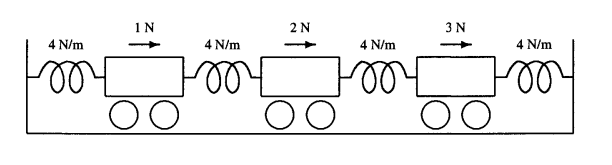
\includegraphics{1020010}
		\caption{}		
		\label{fig:1.4}
	\end{figure}
	Example 1.2.10\\
	\\
	Now suppose we have three masses attached by springs as shown 
	in Figure 1.4. Let $x_1$, $x_2$, and $x_3$ denote the amount by which carts 1, 2, and 3, 
	respectively, move when the forces are applied.\\
	\\
	For each cart the new equilibrium position is that point at which the sum of the forces on the cart is zero. Consider the second cart, for example. An external force of two newtons is applied, and there is 
the leftward force of the spring to the left, and the rightward force of the spring to the right. The amount by which the spring on the left is stretched is $x_2 - x_1$ meters.\\
	\\ 
	It therefore exerts a force $-4$ newtons/meter $\times (x_2 - x_1)$ meters $= -4(x_2 - x_1)$ newtons on the second cart. Similarly the spring on the right applies a force of $+4(x_3 - x_2)$ newtons.\\
	\\
	Thus the equilibrium equation for the second cart is 
	$$-4(x_2-x_1)+4(x_3-x_2)+2=0$$
	or
	$$-4x_1+8x_2-4x_3=2$$
	Similar equations apply to carts 1 and 3. Thus we obtain a system of three linear equations in three unknowns, which we can write as a matrix equation
	\begin{align*}
	\begin{bmatrix}8&-4&0\\-4&8&-4\\0&-4&8\end{bmatrix} \begin{bmatrix} x_1\\x_2\\x_3 \end{bmatrix} = 
	\begin{bmatrix}1\\2\\3\end{bmatrix}
	\end{align*}	
	\\
	Entering the matrix $A$ and vector $b$ into MATLAB, and using the command $x = A\backslash b$ (or simply solving the system by hand) we find that 
	$$b = \begin{bmatrix}0.625\\1.000\\0.875\end{bmatrix}$$
	\\
	Thus the first cart is displaced to the right by a distance of 0.625 meters, for example. The coefficient matrix A is called a stiffness matrix, because the values of its nonzero entries are determined by the stiffnesses of the springs.
	\\
	\\	
	Exercise 1.4.68\\
	\\
	(a) When a spring is stretched (or compressed) from its equilibrium position (0 
	meters) to some new position (x meters), the energy stored in the spring (strain 
	energy) is equal to the work required to move the spring to its new position.\\
	\\ 
	This is $\int_{0}^{x}{f(s)ds}$ joules, the integral of force with respect to distance, where 
	$f(s)$ is the force (in newtons) exerted against the spring that has been stretched 
	to $s$ meters.\\
	\\
	Show that for a linear spring with stiffness $k$ newtons/meter, the 
	strain energy is $\frac{1}{2}kx^2$ joules.\\ 
	\\
	(b) Show that if a spring is stretched or compressed by displacing its right and left 
	endpoints by $x_2$ and $x_1$ meters, respectively, the strain energy of the spring is 
	$\frac{1}{2}k(x_1 - x_2)^2$ joules, which is positive unless $x_1 = x_2$. Show that the strain 
	energy can also be written in the form
	$$\frac{1}{2} * \begin{bmatrix}x_1&x_2\end{bmatrix} \begin{bmatrix}k&-k\\-k&k\end{bmatrix} \begin{bmatrix}x_1\\x_2\end{bmatrix}$$\\
	\\
	(c) Show that the total strain energy of the mass-spring system in Example 1.2.10 
	is a sum of terms of the form $kx^2$ and $k(x_i - x_{i+1}$ and is positive unless all 
	of the displacements are zero.\\
	\\
	(d) Let $A$ be the coefficient matrix of the mass-spring system of Example 1.2.10. 
	Show that the strain energy of the system is $\frac{1}{2}x^TAx$. Deduce that A is positive 
	definite.\\ 
	\\
	(e) Show that the coefficient matrix of the mass-spring system of Exercise 1.2.20 is positive definite. 1.2.20 is the generalization of 1.2.10\\
	\begin{align*}
		\begin{bmatrix}
		k_1+k_2&-k_2&0&...&0\\
		-k_1&k_2+k_3&-k_3&...&0\\
		\vdots&\vdots&\vdots&\vdots&\vdots\\
		...&0&0&-k_{i-1}&k_{i-1}+k_i
		\end{bmatrix}
	\end{align*}
	\\
	Answers:\\
	\\
	(a)\\
	\\
	The applied force varies with the distance and the spring stiffness, so: $f(s)=ks$.
	\begin{align*}
		\int_{0}^{x}{ks\mathrm{d}s} &= k\int_{0}^{x}{s\mathrm{d}s} = k\frac{s^2}{2}\Big|_0^x = k(\frac{x^2}{2}-\frac{0^2}{2}) = k(\frac{x^2}{2})\\
		&=\frac{kx^2}{2}\\
		\square
	\end{align*}
	\\
	(b)\\
	\\
	\begin{align*}
		\int_{0}^{x1-x2}{ks\mathrm{d}s} = k\frac{s^2}{2}\Big|_{0}^{x_1-x_2} =
		k(\frac{(x_1-x_2)^2}{2}) - k(\frac{0^2}{2}) = \frac{k}{2}(x_1-x_2)^2
		\\
		\frac{k}{2}(x_1-x_2)^2\\
		\\
		\begin{bmatrix}x_1&x_2\end{bmatrix}
		\begin{bmatrix}1&-1\\-1&1\end{bmatrix}
		\begin{bmatrix}x_1\\x_2\end{bmatrix} =		
		\begin{bmatrix}x_1-x_2&-x_1+x_2\end{bmatrix}		\begin{bmatrix}x_1\\x_2\end{bmatrix}\\
		= (x_1-x_2)x_1+(-x_1+x_2)x_2\\
		= x_1^2-x_1x_2-x_1x_2+x_2^2\\
		= x_1^2-2x_1x_2+x_2^2\\
		= (x_1-x_2)^2\\
		\\
		\frac{k}{2}\begin{bmatrix}x_1&x_2\end{bmatrix}		\begin{bmatrix}1&-1\\-1&1\end{bmatrix}\begin{bmatrix}x_1\\x_2\end{bmatrix}\\
		= \frac{1}{2} \begin{bmatrix}x_1&x_2\end{bmatrix}	
		\begin{bmatrix}k&-k\\-k&k\end{bmatrix}\begin{bmatrix}x_1\\x_2\end{bmatrix}\\
		\square
	\end{align*}
	\\
	(c)\\
	\\
	We have four springs and the energy in each of them is given by $\frac{1}{2}kx^2$. Each spring has a stifness equal to $4$. So\\
	\begin{align*}
		\frac{1}{2}*4*0.625^2 + \frac{1}{2}*4*(1-0.625)^2+\frac{1}{2}*4*(0.875-1)^2+\frac{1}{2}*4*0.875^2\\
		= 5.25
	\end{align*}
	Stifness is alway positive.\\
	$(x_i)^2$ andd $(x_i - x_{i+1})^2$ are alwyas positive.
	The expression is a sum of positive numbers. The unique exception is when all displacements are zero, when the result is zero.\\
	\\
	(d.1)\\
	\\
	\begin{align*}
		\frac{1}{2}*k_1*x_1^2 + \frac{1}{2}*k_2*(x_2-x_1)^2+\frac{1}{2}*k_3*(x_3-x_2)^2+\frac{1}{2}*k_4*x_3^2\\
		\frac{1}{2}(k_1x_1^2+k_2(x_2-x_1)^2+k_3(x_3-x_2)^2+k_4x_3^2)\\	
	\end{align*}
		\\
	We can also rewrite this as\\
	\\
	\begin{align*}
	x_0 = 0\\
	x_4 = 0\\
	\frac{1}{2}(\sum_{1}^{4}{k_i(x_i-x_{i-1})^2})
	\end{align*}
	Using Octave and Sympy we have:\\
	\begin{verbatim}
	octave:1> pkg load Symbolic;
	octave:2> symbols x1 x2 x3 k1 k2 k3 k4;
	octave:3> expand(k1*x1**2+k2*(x2-x1)**2+k3(x3-x2)**2+k4*x3**2)
	ans = (sym)
     2        2                     2        2                     2        2
	k1*x1  + k2*x1  - 2*k2*x1*x2 + k2*x2  + k3*x2  - 2*k3*x2*x3 + k3*x3  + k4*x3
	octave:4> latex(ans)
	k_{1} x_{1}^{2} + k_{2} x_{1}^{2} - 2 k_{2} x_{1} x_{2} + k_{2} x_{2}^{2} 
	+ k_{3} x_{2}^{2} - 2 k_{3} x_{2} x_{3} + k_{3} x_{3}^{2} + k_{4} x_{3}^{2}
	\end{verbatim}
	Which gives us :\\
	\begin{align*}
	k_{1} x_{1}^{2} + k_{2} x_{1}^{2} - 2 k_{2} x_{1} x_{2} + k_{2} x_{2}^{2} + k_{3} x_{2}^{2} - 2 k_{3} x_{2} x_{3} + k_{3} x_{3}^{2} + k_{4} x_{3}^{2}
	\end{align*}
	Using Octave and Sympy again we see that we can rewrite this expression as:\\
	\begin{verbatim}
	octave:5> expand([x1,x2,x3]*[k1+k2,-k2,0;-k2,k2+k3,-k3;0,-k3,k3+k4]*[x1;x2;x3])
	ans = (sym)
		    2        2                     2        2                     2        2
	k1*x1  + k2*x1  - 2*k2*x1*x2 + k2*x2  + k3*x2  - 2*k3*x2*x3 + k3*x3  + k4*x3
	octave:6> latex(ans)
	k_{1} x_{1}^{2} + k_{2} x_{1}^{2} - 2 k_{2} x_{1} x_{2} + k_{2} x_{2}^{2}
	+ k_{3} x_{2}^{2} - 2 k_{3} x_{2} x_{3} + k_{3} x_{3}^{2} + k_{4} x_{3}^{2}
	\end{verbatim}
	Which is exactly what we had earlier.
	\begin{align*}
	k_{1} x_{1}^{2} + k_{2} x_{1}^{2} - 2 k_{2} x_{1} x_{2} + k_{2} x_{2}^{2}
	+ k_{3} x_{2}^{2} - 2 k_{3} x_{2} x_{3} + k_{3} x_{3}^{2} + k_{4} x_{3}^{2}
	\end{align*}
	So, we can write the Straing Energy of the system as\\
	\begin{align*}
	E &=
	\frac{1}{2} *
	\begin{bmatrix}x_1&x_2&x_3\end{bmatrix}
	\begin{bmatrix}k_1+k_2&-k_2&0\\-k_2&k_2+k_3&-k_3\\0&-k_3&k_3+k_4\end{bmatrix}
	\begin{bmatrix}x_1\\x_2\\x_3\end{bmatrix}\\
	E &= \frac{1}{2}x^TAx
	\end{align*}
	\\
	(d.2) and (e)\\
	\\
	Now we can show that A is "Positive Definite":\\
	\begin{align*}
		A = \begin{bmatrix}k_1+k_2&-k_2&0\\-k_2&k_2+k_3&-k_3\\0&-k_3&k_3+k_4\end{bmatrix}\\
	\end{align*}
	\\
	Using the summation expression from above, we can generalize A to the (e) part of the question and answer both at the same time.\\
	First the easy part:\\
	1) A is Square\\
	2) A is symmetric\\  we have:
	\begin{align*}
		x^tAx &> 0\\
		x^tAx &= \\
		&x_0 = 0\\
		&x_{i+1} = 0\\
		&\frac{1}{2}(\sum_{1}^{i+1}{k_i(x_i-x_{i-1})^2})
	\end{align*}
	But all $k_i$ are positive.\\
	All $(x_i-x_{i-1})^2$ are positive.\\
	So the summation of positive is positive.\\
	Half of positive is positive, so:
	\begin{align*}
		x^tAx &> 0\\
	\end{align*}
	What makes $A$ "Positive Definite".\\
	$\square$
\end{document}